\section{MPI Implementation}
\label{sec:mpi}

The MPI version follows a completely different strategy. This was entirely based on the article [\cite{paper}].

For this implementation, it is assumed that each process owns a partition of the array, and that all partitions are equal in size. Also, like the OpenMP version, each bucket is assigned to a single process. So for $B$ buckets, a maximum of $P$ processes should be used, otherwise no significant improvements would happen.

The general workflow for each iteration is:

\begin{enumerate}
	\item \textbf{Local Bucket fill}. Each process creates a list of buckets indexing its local partition. An auxiliary array of size $B$ is also created, containing the size of each local bucket.

	\item \textbf{\emph{all-to-all} transpose}. Each process will now need information about the size buckets that are assigned to them. For instance, if process 0 is handling bucket 0, then all other processes will be required to inform him about the size of their local bucket 0. The global bucket 0 will have a size equal to the sum of each local one. This operation is more clearly shown in \autoref{fig:mpi}

	\item \textbf{Communication}. Knowing how many elements each bucket will have, every process will now send the keys to the apropriate destinations
\end{enumerate}

\begin{figure}[!htpb]
	\begin{center}
		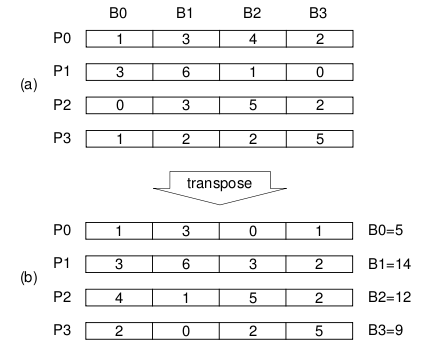
\includegraphics[width=0.45\textwidth]{images/mpi}
	\end{center}
	\caption{\emph{all-to-all} transpose operation. (a) shows the local bucket sizes in each proc. With eack bucket being assigned to one process, the transpose of this, being shown in (b) ilustrates the wanted result}
	\label{fig:mpi}
\end{figure}

Besides ilustrating how the transpose operation works, \autoref{fig:mpi} also happens to expose the problem with this implementation, which is load balancing. For example, after the iteration shown, P0 will have 5 elements on its local partition, and P1 will have 14. The next iteration will give completely different values for each process, since each iteration is based on an entirely different digit. Not only is the amount of elements per process completely unbalanced, the communication is also a problem.
